\documentclass{article}

% TODO: for final version, see the TODOs below: we commented out sections to make them anonymous

% if you need to pass options to natbib, use, e.g.:
%     \PassOptionsToPackage{numbers, compress}{natbib}
% before loading neurips_2026

% The authors should use one of these tracks.
% Before accepting by the NeurIPS conference, select one of the options below.
% 0. "default" for submission
% \usepackage{neurips_2026}
% the "default" option is equal to the "main" option, which is used for the Main Track with double-blind reviewing.
% 1. "main" option is used for the Main Track
%  \usepackage[main]{neurips_2026}
% 2. "position" option is used for the Position Paper Track
%  \usepackage[position]{neurips_2026}
% 3. "eandd" option is used for the Evaluations & Datasets Track
 % \usepackage[eandd]{neurips_2026}
% 4. "creativeai" option is used for the Creative AI Track
%  \usepackage[creativeai]{neurips_2026}
% 5. "sglblindworkshop" option is used for the Workshop with single-blind reviewing
 % \usepackage[sglblindworkshop]{neurips_2026}
% 6. "dblblindworkshop" option is used for the Workshop with double-blind reviewing
%  \usepackage[dblblindworkshop]{neurips_2026}

% After being accepted, the authors should add "final" behind the track to compile a camera-ready version.
% 1. Main Track
 % \usepackage[main, final]{neurips_2026}
% 2. Position Paper Track
%  \usepackage[position, final]{neurips_2026}
% 3. Evaluations & Datasets Track
 % \usepackage[eandd, final]{neurips_2026}
% 4. Creative AI Track
%  \usepackage[creativeai, final]{neurips_2026}
% 5. Workshop with single-blind reviewing
%  \usepackage[sglblindworkshop, final]{neurips_2026}
% 6. Workshop with double-blind reviewing
%  \usepackage[dblblindworkshop, final]{neurips_2026}
% Note. For the workshop paper template, both \title{} and \workshoptitle{} are required, with the former indicating the paper title shown in the title and the latter indicating the workshop title displayed in the footnote.
% For workshops (5., 6.), the authors should add the name of the workshop, "\workshoptitle" command is used to set the workshop title.
% \workshoptitle{WORKSHOP TITLE}

% "preprint" option is used for arXiv or other preprint submissions
 % \usepackage[preprint]{neurips_2026}

% to avoid loading the natbib package, add option nonatbib:
\usepackage[nonatbib]{neurips_2026}

\usepackage[utf8]{inputenc} % allow utf-8 input
\usepackage[T1]{fontenc}    % use 8-bit T1 fonts
% I removed this one: \usepackage{hyperref}       % hyperlinks
\usepackage{url}            % simple URL typesetting
\usepackage{booktabs}       % professional-quality tables
\usepackage{amsfonts}       % blackboard math symbols
\usepackage{nicefrac}       % compact symbols for 1/2, etc.
\usepackage{microtype}      % microtypography
\usepackage{xcolor}         % colors

%% I added the following packages and shortcuts
\usepackage[hidelinks,colorlinks=true,linkcolor=blue,citecolor=blue,urlcolor=blue]{hyperref}
\usepackage{amsmath}
\usepackage{amssymb}
\usepackage{graphicx}
\usepackage{makecell}
\usepackage{multirow}
%\usepackage{tablefootnote}
\usepackage{enumitem}
\usepackage{pythonhighlight}  % for python listings
\usepackage[numbers]{natbib}
\usepackage{caption}
\captionsetup[figure]{skip=5pt}  % reduce the space between figure and caption
%\captionsetup[table]{skip=10pt}  % default is 10pt
\usepackage{amsthm}
\newtheorem{proposition}{Proposition}
\newtheorem{corollary}{Corollary}
\newtheorem{remark}{Remark}

% shortcuts
\newcommand{\mat}[1]{\mathbf{#1}}     % shortcut for matrix
\newcommand{\RMS}[1]{\text{RMS}(#1)}  % shortcut for RMS(x)
\def\rms{\text{RMS}(\vec{a})}         % RMS(a)
\def\f1n{\frac{1}{n}}                 % 1/n
\def\sas{\sum_{i=1}^n a_i^2}           % sum over a_i squared
\def\W*{\mat{W}^\ast}                 % matrix W*
\def\V*{\mat{V}^\ast}                 % matrix V*
\def\mW{\mat{W}}                      % matrix W
\def\mV{\mat{V}}                      % matrix V
\def\a{\vec{a}}                       % vector a
\def\b{\vec{b}}                       % vector b
\def\c{\vec{c}}                       % vector c
\def\vb{\vec{\beta}}                  % vector beta
\def\vx{\vec{x}}                      % vector x
\def\vy{\vec{y}}                      % vector y
\def\vz{\vec{z}}                      % vector z
\def\vg{\vec{g}}                      % vector g
\def\vs{\vec{s}}                      % vector s
\def\cosi{\cos{(\cdot)}}              % cos(.)
\def\sini{\sin{(\cdot)}}              % sin(.)

% Note. For the workshop paper template, both \title{} and \workshoptitle{} are required, with the former indicating the paper title shown in the title and the latter indicating the workshop title displayed in the footnote.
\title{FlashNorm: Fast Normalization for Transformers}

% The \author macro works with any number of authors. There are two commands
% used to separate the names and addresses of multiple authors: \And and \AND.
%
% Using \And between authors leaves it to LaTeX to determine where to break the
% lines. Using \AND forces a line break at that point. So, if LaTeX puts 3 of 4
% authors names on the first line, and the last on the second line, try using
% \AND instead of \And before the third author name.
\author{%
  David S.~Hippocampus\thanks{Use footnote for providing further information
    about author (webpage, alternative address)---\emph{not} for acknowledging
    funding agencies.} \\
  Department of Computer Science\\
  Cranberry-Lemon University\\
  Pittsburgh, PA 15213 \\
  \texttt{hippo@cs.cranberry-lemon.edu} \\
  % examples of more authors
  % \And
  % Coauthor \\
  % Affiliation \\
  % Address \\
  % \texttt{email} \\
  % \AND
  % Coauthor \\
  % Affiliation \\
  % Address \\
  % \texttt{email} \\
  % \And
  % Coauthor \\
  % Affiliation \\
  % Address \\
  % \texttt{email} \\
}

\begin{document}

\maketitle

\begin{abstract}
Normalization layers are ubiquitous in large language models (LLMs) yet represent
a compute bottleneck: on hardware with distinct vector and matrix execution
units, the RMS calculation blocks the subsequent matrix multiplication, preventing
parallel execution. We present \textbf{FlashNorm}, an \emph{exact} reformulation of
RMSNorm followed by a linear layer that (i) eliminates the normalization weights
by folding them into the subsequent linear layer, and (ii) defers the scalar
RMS normalization to the output of the matrix multiplication, enabling the two
operations to execute in parallel.
The same techniques extend to LayerNorm and  Dynamic Tanh (DyT).
And due to RMS scale invariance, a linear layer between two RMSNorms makes the
first one redundant, removing the pre-attention RMSNorm in QKV-normalized models
(e.g., Gemma~4) and in MLA-models
with latent normalization (e.g., DeepSeek-V2, Mistral Small 4).
On an NVIDIA T4 GPU, FlashNorm achieves \textbf{33--35\%}
lower latency on the norm-then-project operation in the compute-bound (prefill)
regime at SmolLM2-135M scale, and \textbf{12--14\%} at Llama-7B scale.
On an NVIDIA A100, FlashNorm achieves a \textbf{13\%} end-to-end speedup
at decode on Llama-3.2-1B in HuggingFace Transformers.
We verify zero-loss weight folding on three models.
Beyond inference speed, FlashNorm simplifies model implementations by
reducing parameter tensor count.
\end{abstract}

\begin{figure}[h!] \centering  % the [h!] tries to place the picture right here
  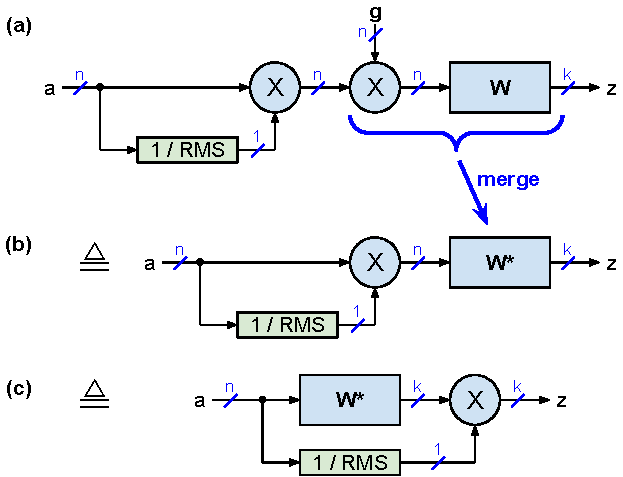
\includegraphics[scale=0.8]{../doc/fig/flashNorm_fig1.pdf}
  \caption{Mathematically identical implementations of RMSNorm followed by a linear layer.
    (a) Standard: normalization weights $\mathbf{g}$ are applied element-wise before $\mathbf{W}$.
    (b) \textbf{Weightless}: $\mathbf{g}$ is folded into $\mathbf{W}^* = \mathrm{diag}(\mathbf{g})\mathbf{W}$.
    (c) \textbf{FlashNorm}: normalization is deferred to the output, enabling matrix multiplication
    ($\mathbf{W}^*$) and RMS calculation to execute in parallel. $\triangleq$ denotes
    mathematical identity.}
\label{fig1} \end{figure}

\section{Introduction}
Normalization is indispensable to the training stability and generalization of
modern LLMs. RMSNorm~\citep{rms}, used by Llama~\citep{LLaMA},
Gemma~\citep{gemma}, Mistral~\citep{mistral}, and
OLMo~2~\citep{olmo2}, normalizes each activation vector by its root mean
square (RMS) before scaling by learned weights. In the standard transformer network~\citep{vanilla},
RMSNorm is followed immediately by a linear (projection) layer---in both the attention and
feed-forward sub-networks of every transformer block.

This sequential structure conceals a hardware inefficiency. On processors with
dedicated vector units (for element-wise ops) and matrix units (for matrix multiplication), the
RMS value must be fully computed \emph{before} the linear layer can begin, because
the normalized activations are its input. The matrix unit therefore sits idle during
the RMS calculation, a bottleneck that compounds across all transformer layers and inference calls.

We address this bottleneck with \textbf{FlashNorm}, which makes two
mathematically equivalent transformations to the RMSNorm-then-project pipeline shown in
Fig.~\ref{fig1}(a):

\begin{enumerate}
  \item \textbf{Weightless normalization.} The per-channel normalization weights
        $\mathbf{g}$ are absorbed into the weight matrix of the following linear layer,
        eliminating them as a separate parameter tensor as illustrated in Fig.~\ref{fig1}(b).
  \item \textbf{Deferred normalization.} Because scaling by $1/\mathrm{RMS}(\mathbf{a})$
        commutes with matrix multiplication, the scalar normalization is
        moved to the \emph{output} of the linear layer as shown in Fig.~\ref{fig1}(c).
        This allows the matrix multiplication and the RMS calculation to execute in parallel on separate
        hardware units.
\end{enumerate}

The name is inspired by FlashAttention \citep{flash-attention}, where the
softmax denominator is similarly deferred past a matrix multiplication to enable
parallel processing of keys and values.

FlashNorm requires no retraining, and weight folding can be applied post-hoc to any pretrained
checkpoint. We further show how the same ideas extend to Layer Normalization~\citep{layerNorm},
DyT~\citep{DyT}, GLU-variant FFNs~\citep{GLU}, and RoPE-based attention~\citep{RoPE}.

\paragraph{Contributions.}
\begin{itemize}
  \item We formally characterize the commutativity of RMSNorm with
        matrix multiplication (Proposition~\ref{prop:commute}) and derive
        the exact conditions under which deferred normalization holds.
  \item We show that RMS scale invariance allows an RMSNorm--linear--RMSNorm
        sequence to drop the first RMSNorm entirely (Proposition~\ref{prop:rms-cancel}),
        eliminating the pre-attention RMSNorm in models with QKV-normalization \citep{qkv-norm}
        such as Gemma~4 \citep{gemma4} and in MLA-models with latent normalization
        (e.g., DeepSeek-V2 \citep{deepseek-v2},
        Mistral Small 4 \citep{mistral4}, OpenMythos \citep{openMythos}).
  \item We present FlashNorm as a unified framework covering RMSNorm, LayerNorm,
        DyT, GLU-FFNs, and attention with RoPE.
  \item We verify zero-loss weight-folding on SmolLM2-135M, Llama-3.2-1B, and
        Llama-3.1-8B across wikitext, MMLU, and HellaSwag (Table~\ref{tab:quality}),
        and report operation-level speedups on T4, A100, and H100.
  \item And we identify the kernel-engineering work required to extend to
        compute-bound regimes and provide a reference design.
\end{itemize}

\section{Background and Related Work}

\paragraph{Normalization in transformers.}
Layer Normalization~\citep{layerNorm} applies mean centering followed by
variance normalization with learned scale and bias. RMSNorm~\citep{rms}
drops mean centering and bias, reducing to pure RMS-based scaling; it has become the
dominant normalization choice in recent open LLMs due to its simplicity and
comparable empirical performance. Dynamic Tanh (DyT)~\citep{DyT} is a
recently proposed drop-in replacement that eliminates the normalization computation
entirely, replacing it with a parameterized $\tanh$; FlashNorm is complementary in
that it targets the interaction between normalization and the subsequent linear layer.

\paragraph{Kernel fusion and operation reordering.}
Fusing small operations into a single GPU kernel is a standard optimization to
reduce memory bandwidth and kernel-launch overhead. \citet{openelm} report
that modifications to the layer normalization implementation significantly affect
tokens-per-second throughput, attributing this to a lack of kernel fusion. FlashNorm
reduces the number of kernel launches by eliminating the normalization weight
application as a separate step, and additionally enables parallelism between the
vector and matrix units that kernel fusion alone cannot achieve.

\paragraph{Weight folding and parameter elimination.}
The idea of absorbing one layer's parameters into a neighboring layer appears in
several forms. Batch normalization folding into convolutional weights is standard
practice in quantization-aware training and model deployment~\citep{quantJacob, convBN}
and \verb+torch.compile+ can perform it automatically~\citep{torchCompileFuse}.
OLMo~1 models use weightless LayerNorm, which they call
\emph{non-parametric}~\citep{olmo2}. FlashNorm applies analogous reasoning to
normalization weights of RMSNorm and LayerNorm.

\paragraph{FlashAttention.}
FlashAttention~\citep{flash-attention} is the closest conceptual predecessor:
it defers the softmax normalization (division by $\sum \exp$) past the multiplication
with the value matrix $\mathbf{V}$, enabling online computation and improving memory
efficiency. FlashNorm applies the same reordering insight to the simpler setting of
RMSNorm and a dense linear layer.

\section{FlashNorm}
We now develop FlashNorm formally. All propositions assume bias-free linear layers
unless stated otherwise; Section~\ref{sec:bias} addresses the biased case.

\subsection{Weightless Normalization}
Let $\mathbf{a} \in \mathbb{R}^n$ be an activation vector. RMSNorm computes
\[
  \mathrm{RMSNorm}(\mathbf{a})_i = \frac{a_i}{\mathrm{RMS}(\mathbf{a})} \cdot g_i,
  \qquad
  \mathrm{RMS}(\mathbf{a}) = \sqrt{\frac{1}{n}\sum_{i=1}^n a_i^2},
\]
where $\mathbf{g} \in \mathbb{R}^n$ are learned normalization weights.
In transformer models, RMSNorm is followed by a linear layer $\mathbf{W} \in \mathbb{R}^{n \times k}$  as illustrated in Fig. \ref{fig1}(a):
\[
  \mathbf{z} = \mathrm{RMSNorm}(\mathbf{a})\, \mathbf{W}.
\]

\begin{proposition}[Weightless normalization]\label{prop:weightless}
Let $\mathbf{W}^* \in \mathbb{R}^{n \times k}$ be defined by $W^*_{i,j} = g_i \cdot W_{i,j}$.
Then $\mathbf{z} = \frac{\mathbf{a}}{\mathrm{RMS}(\mathbf{a})}\, \mathbf{W}^*$, i.e.,
the normalization weights $\mathbf{g}$ can be absorbed into $\mathbf{W}$ and need not
be stored or applied separately.
\end{proposition}

\begin{proof}
$z_j = \sum_i \frac{a_i}{\mathrm{RMS}(\mathbf{a})} g_i W_{i,j}
     = \sum_i \frac{a_i}{\mathrm{RMS}(\mathbf{a})} W^*_{i,j} $.
\end{proof}

This proposition holds for linear layers with or without a bias term at the output.
The practical implication is that the normalization weight vector $\mathbf{g}$ becomes
a redundant parameter: it can be folded into $\mathbf{W}$ once at load time, saving
memory, reducing the parameter count, and eliminating one vector-multiply kernel call
per forward pass.

\subsection{Deferred Normalization}

\begin{proposition}[Commutativity of RMS scaling with matrix multiplication]\label{prop:commute}
Let $\mathbf{W}^*$ be as in Proposition~\ref{prop:weightless} and let the linear
layer be bias-free. Then
\[
  \mathbf{z}
  = \frac{\mathbf{a}}{\mathrm{RMS}(\mathbf{a})}\,\mathbf{W}^*
  = (\mathbf{a}\,\mathbf{W}^*)\cdot \frac{1}{\mathrm{RMS}(\mathbf{a})}.
\]
That is, the scalar normalization $1/\mathrm{RMS}(\mathbf{a})$ can be applied
\emph{after} the matrix multiplication.
\end{proposition}

\begin{proof}
Scalar multiplication commutes with matrix multiplication:
$(\alpha \mathbf{a})\mathbf{W}^* = (\mathbf{a}\mathbf{W}^*) \alpha$ for any scalar
$\alpha$. Setting $\alpha = 1/\mathrm{RMS}(\mathbf{a})$ gives the result.
\end{proof}

\begin{corollary}[Parallel execution]\label{cor:parallel}
Under the conditions of Proposition~\ref{prop:commute}, computing
$\mathbf{a}\mathbf{W}^*$ and $\mathrm{RMS}(\mathbf{a})$ are \emph{independent}
computations that may proceed in parallel. The final result requires only a single
vector-scalar multiply after both complete.
\end{corollary}

\begin{remark}[Bias case]
If the linear layer has a bias $\mathbf{c} \in \mathbb{R}^k$, deferred normalization
does not hold directly because
$(\mathbf{a}\mathbf{W}^* + \mathbf{c}) / \mathrm{RMS}(\mathbf{a}) \neq
 \mathbf{a}\mathbf{W}^*/\mathrm{RMS}(\mathbf{a}) + \mathbf{c}$.
In this case, Proposition~\ref{prop:weightless} (weightless normalization) still
applies, but the normalization must precede the bias addition.
% TODO(nils): clarify that in this case we can still compute RMS and matmul in parallel!
\end{remark}

\begin{remark}[Unfolded case]
Proposition~\ref{prop:commute} requires only that $1/\mathrm{RMS}(\mathbf{a})$ be a per-token scalar. Propositions~\ref{prop:weightless} and~\ref{prop:commute} are therefore independent: a framework implementing deferred normalization alone obtains the parallel-execution and fused-kernel speedups (Corollary~\ref{cor:parallel} and Appendix~\ref{app:a100}) for any existing RMSNorm checkpoint, with no weight-folding required.
\end{remark}

Figure~\ref{fig1} illustrates the three mathematically equivalent
implementations: (a) standard RMSNorm-then-project, (b) weightless normalization,
and (c) the full FlashNorm with deferred normalization.

\subsection{Cancellation of Pre-Normalization}\label{sec:rms-cancel}

\begin{proposition}[RMSNorm cancellation]\label{prop:rms-cancel}
For activation $\mathbf{a}$, linear layer $\mathbf{W}^*$ (with normalization weights
already folded in as per Proposition~\ref{prop:weightless}), and a second RMSNorm
applied to the output,
\[
  \mathrm{RMSNorm}\!\left(\frac{\mathbf{a}}{\mathrm{RMS}(\mathbf{a})}\,\mathbf{W}^*\right)
  = \mathrm{RMSNorm}\!\left(\mathbf{a}\,\mathbf{W}^*\right),
\]
i.e., the first RMSNorm is redundant and can be eliminated entirely as shown in Fig. \ref{fig6}.
\end{proposition}
\begin{proof}
Let $\mathbf{b} = \mathbf{a}\mathbf{W}^*$, $s_a = 1/\mathrm{RMS}(\mathbf{a})$, and
$\mathbf{c} = \mathbf{b} \cdot s_a$, see Fig. \ref{fig6}.  By scale invariance of RMS,
$\mathrm{RMS}(\mathbf{c}) = s_a \cdot \mathrm{RMS}(\mathbf{b})$, so the product of the two scalers $s_a$
and $\frac{1}{\mathrm{RMS}(\mathbf{c})}$ is $s_a \cdot \frac{1}{\mathrm{RMS}(\mathbf{c})}
= s_a \cdot \frac{1}{s_a \cdot \mathrm{RMS}(\mathbf{b})} = \frac{1}{\mathrm{RMS}(\mathbf{b})}$,
and therefore $\mathrm{RMSNorm}(\mathbf{c}) = \mathrm{RMSNorm}(\mathbf{b})$.
\end{proof}
\paragraph{Eliminating pre-attention RMSNorm with QKV-normalization.}
Some models such as Gemma~4 \citep{gemma4} apply QKV-normalization~\citep{qkv-norm} to
queries, keys, \emph{and values}. The sequence is:
pre-attention RMSNorm $\to$ QKV-projection $\to$ QKV-RMSNorm.
By Proposition~\ref{prop:rms-cancel}, the pre-attention RMSNorm cancels and can be
dropped entirely, saving one full RMSNorm per each transformer block.

\paragraph{Eliminating pre-attention RMSNorm with MLA latent normalization.}
The sequence for MLA with latent normalization is:
pre-attention RMSNorm $\to$ down-projection into latent space $\to$ latent RMSNorm,
which matches the pattern of Proposition~\ref{prop:rms-cancel} exactly.
The pre-attention RMSNorm therefore cancels and can be eliminated.
This optimization applies to all the MLA models we inspected, including
DeepSeek-V2 \citep{deepseek-v2}, Mistral Small 4 \citep{mistral4}, and
OpenMythos \citep{openMythos}.

\paragraph{Epsilon caveat.}
The scale-invariance $\mathrm{RMS}(s\cdot\mathbf{a}) = s\cdot\mathrm{RMS}(\mathbf{a})$ does
not hold exactly for the $\varepsilon$-regularized variant
$\mathrm{RMS}_\varepsilon(\mathbf{a}) = \sqrt{\varepsilon + \frac{1}{n}\sum a_i^2}$.
The discrepancy is negligible in practice: $\varepsilon$ only has material effect when the
activation energy is near zero, where it limits up-scaling, see appendix.
\begin{figure}[h!] \centering
  \includegraphics[scale=0.8]{../doc/fig/flashNorm_fig6.pdf}
  \caption{Weightless RMSNorm followed by a linear layer and a second RMSNorm:
    (a) unoptimized version; (b) optimized version where the first RMSNorm is
    eliminated by Proposition~\ref{prop:rms-cancel}.}
\label{fig6} \end{figure}

\subsection{Support for Normalization Bias}\label{sec:bias}
LayerNorm~\citep{layerNorm} and DyT~\citep{DyT} include an additive
bias $\boldsymbol{\beta}$ after scaling by $\mathbf{g}$. Fig. \ref{figA}
illustrates how this bias can be moved to
the output of the following linear layer, resulting in a modified bias
$\mathbf{c}^* = \mathbf{c} + \boldsymbol{\beta}\mathbf{W}$, see Fig. \ref{figA}(b).
After this elimination of $\boldsymbol{\beta}$, the normalization weights
$\mathbf{g}$ can be folded into the linear layer as per Proposition~\ref{prop:weightless}.
Note that deferred normalization (Proposition~\ref{prop:commute}) does not apply
when a bias is present; the scalar $1/\mathrm{RMS}(\mathbf{a})$ must be applied
before adding $\mathbf{c}^*$, which still allows for parallel execution of matrix
multiplication and RMS calculation.

\begin{figure}[h!] \centering  % the [h!] tries to place the picture right here
  \includegraphics[scale=0.8]{../doc/fig/flashNorm_figA.pdf}
  \caption{Elimination of bias $\boldsymbol{\beta}$: (a) Before elimination with $\boldsymbol{\beta}$
    between normalization weights $\mathbf{g}$ and linear layer. (b) Optimized version with new
    bias term $\mathbf{c}^* = \mathbf{c} + \boldsymbol{\beta}\mathbf{W}$ at the output.}
\label{figA} \end{figure}

\subsection{Folding Mean Centering into a Preceding Linear Layer}
LayerNorm applies mean centering before RMSNorm. If mean centering is preceded by a
linear layer with weights $\mathbf{V} \in \mathbb{R}^{n \times n}$, the centering
can be absorbed into $\mathbf{V}$ without retraining, see Fig. \ref{figB}: The mean $\mu$ is
calculated from the linear layer outputs $y_j$ as
$\mu = \frac{1}{n} \sum_j y_j$ where $y_j = \sum_i x_i V_{i,j}$.
Let $s_i = \sum_j V_{i,j}$ be the row sum of row $i$, we can then
calculate $\mu$ directly from the inputs $x_i$ as
\begin{equation*}
  \mu = \frac{1}{n} \sum_{j=1}^n \sum_{i=1}^n x_i V_{i,j} = \frac{1}{n} \sum_{i=1}^n x_i \left[ \sum_{j=1}^n V_{i,j} \right] = \frac{1}{n} \sum_{i=1}^n x_i s_i .
\end{equation*}
The mean-centered outputs are now
\begin{equation*}
  a_j = y_j - \mu = \sum_{i=1}^n x_i V_{i,j} - \frac{1}{n} \sum_{i=1}^n x_i s_i
       = \sum_{i=1}^n x_i \underbrace{\left( V_{i,j} - \frac{s_i}{n} \right)}_{V^*_{i,j}},
\end{equation*}
so the modified weights $V^*_{i,j} = V_{i,j} - s_i/n$ absorb the mean centering
entirely, see Fig. \ref{figB}(b). This also provides a lossless recipe for converting a LayerNorm model
to RMSNorm without any retraining.
\begin{figure}[h!] \centering  % the [h!] tries to place the picture right here
  \includegraphics[scale=0.8]{../doc/fig/flashNorm_figB.pdf}
  \caption{Elimination of mean centering: (a) Original weight matrix $\mV$ followed by mean centering. (b) Optimized version where the mean centering is merged into the modified weight matrix $\V*$.}
\label{figB} \end{figure}

\section{Extensions}

\subsection{FlashNorm for FFNs with GLU Variants}
For GLU-variant FFNs~\citep{GLU}, the FlashNorm at the FFN
input requires scaling at both the Gate and Up projection outputs, see Fig. \ref{fig3}(a).
One of these scaling operations can be deferred to the FFN output, saving $f - n$ multiply operations
as shown in Fig. \ref{fig3}(b). See appendix for FFNs with ReLU, ReGLU and Bilinear GLU variants.
\begin{figure}[h!] \centering
  \includegraphics[scale=0.8]{../doc/fig/flashNorm_fig3.pdf}
  \caption{FFN with GLU variant and preceding FlashNorm: (a) unoptimized version; (b) optimized version with fewer scaling multipliers.}
\label{fig3} \end{figure}

\subsection{FlashNorm for Attention with RoPE}
For the query ($\mathbf{Q}^*$) and key ($\mathbf{K}^*$) projections in RoPE-based
attention~\citep{RoPE}, the $1/\mathrm{RMS}(\mathbf{a})$ factor can be
fused with the precomputed RoPE cosine and sine tables, which are shared across
all attention heads as shown in Fig. \ref{fig5}.
Specifically, replacing $\cos(\cdot)$ with
$\cos(\cdot)/\mathrm{RMS}(\mathbf{a})$ (and similarly for $\sin$) eliminates the
per-head scaling entirely, saving $2hH - h$ multiply operations, where $h$ is the head
dimension and $H$ is the number of heads. Additionally, the $1/\sqrt{h}$ scaled
dot-product factor can be folded into the same scaling operation.
\begin{figure}[h!] \centering
  \includegraphics[scale=0.8]{../doc/fig/flashNorm_fig5.pdf}
  \caption{FlashNorm for scaled dot-product attention with RoPE: (a) unoptimized version; (b) optimized version where the normalization is fused with $\cosi$ and $\sini$.}
\label{fig5} \end{figure}

\subsection{QK-Normalization}\label{sec:qknorm}
Gemma~3~\citep{gemma3}, OLMo~2~\citep{olmo2}, OpenELM~\citep{openelm} and other LLMs
use QK-normalization~\citep{QKnorm}, which applies RMSNorm to queries and
keys \emph{after} the projection. Unlike QKV-normalization, V is not normalized, so
the pre-attention RMSNorm cannot be fully eliminated---but the $1/\mathrm{RMS}(\mathbf{a})$
scalers for Q and K can still be dropped via Proposition~\ref{prop:rms-cancel}
(Fig.~\ref{fig7}). Two further optimizations are available:

\paragraph{Fusing QK-norm weights with RoPE.}
If QK-norm weights are shared across all heads of a layer (as in Gemma~3 and
OpenELM), they can be fused with the RoPE cosine and sine vectors, which are
already shared across heads, see Fig. \ref{fig7}.
The fused tables are computed once per layer, and
the normalization weights require only a permutation to align with RoPE's
interleaved layout.

\paragraph{Weight-fusion for NoPE channels.}
Several architectures employ partial RoPE or interleave RoPE and NoPE layers
(e.g., Llama~4~\citep{llama4}). For these models, we can fuse the Q and K normalization
weights for the NoPE channels as
$g_{\mathbf{QK}, i} = g_{\mathbf{Q}, i} * g_{\mathbf{K}, i}$ for $i \in [ \mathrm{NoPE} ]$.
\begin{figure}[h!] \centering
  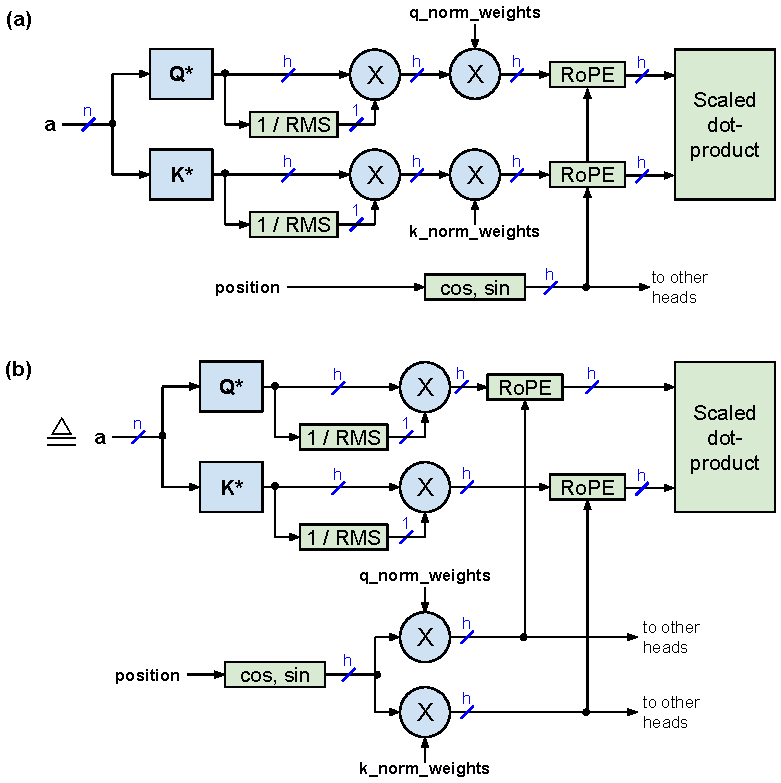
\includegraphics[scale=0.8]{../doc/fig/flashNorm_fig7.pdf}
  \caption{QK-norm with RoPE: (a) unoptimized version; (b) optimized version.}
\label{fig7} \end{figure}

\section{Hardware Analysis}
We analyze the compute bottleneck that FlashNorm eliminates.
Consider a processor with one vector unit
(throughput: $m$ ops/cycle) and one matrix unit (throughput: $m^2$ ops/cycle) where $m$ is the processor width. Specifically:
\begin{itemize}
    \item Multiplying an $n$-vector with an $n \times n$ matrix takes $n^2$ MAD (multiply-add)
          operations, which takes $n^2/m^2$ matrix cycles.
    \item Computing  $1/\mathrm{RMS}(\mathbf{a})$ requires $n$ MAD operations (for squaring and adding)
          plus 2 scalar ops (for $\sqrt{n/x}$), which takes $n/m$ vector cycles if we ignore
          the 2 scalar ops.
    \item Scaling an $n$-vector by a scalar takes $n/m$ vector cycles.
\end{itemize}

Fig.~\ref{fig8} shows timing diagrams for the example $n = 512$ and $m = 128$.
Without FlashNorm (sequential execution), the matrix unit cannot begin until both
the RMS and the scaling are complete, imposing an 8 cycle bubble as shown in Fig.~\ref{fig8}(a).
The subsequent vector-matrix multiply takes $(512)^2 / (128)^2 = 16$ cycles; the total is 24 cycles.
With row-major ordering, the first rows of $\mathbf{W}^*$ can be processed
while later rows of the RMS accumulation are still in flight, reducing the bubble
to 5 cycles (total: 21 cycles), but the bottleneck persists, see Fig.~\ref{fig8}(b).
With FlashNorm, the vector-matrix multiply ($\mathbf{a}\mathbf{W}^*$) and
the RMS calculation proceed fully in parallel on separate units as shown in Fig.~\ref{fig8}(c).
The scaling at the end can be performed in parallel to the matrix unit if $\mat{W}^*$ is processed in column-major order.
Total execution: 17 cycles---a \textbf{29\% reduction} versus the sequential baseline.
\begin{figure}[h!] \centering
  \includegraphics[scale=0.8]{../doc/fig/flashNorm_fig8.pdf}
  \caption{Exemplary timing diagrams.
    (a) Sequential: matrix unit idles 8 cycles.
    (b) Partial overlap with interleaved scaling and vector-matrix multiplication.
    (c) \textbf{FlashNorm}: vector-matrix multiply and RMS run fully in parallel.}
\label{fig8} \end{figure}

\section{Experiments}\label{sec:experiments}
% TODO:
% Refer to \citep{hfFlashNorm, tricks} for Python code that demonstrates the mathematical equivalency of the optimizations presented in this paper.
% A reproducible Colab notebook for the GPU benchmarks below is available in the \verb+transformer-tricks+ repository\footnote{\url{https://github.com/OpenMachine-ai/transformer-tricks/blob/main/notebooks/flashNorm\_gpu\_benchmark.ipynb}}.

We verified lossless weight folding on SmolLM2-135M \citep{smollm}, Llama-3.2-1B, and Llama-3.1-8B \citep{LLaMA}.
% TODO
% using \verb+flashify_repo()+ from the \verb+transformer-tricks+ package \citep{tricks}.
On SmolLM2-135M under HuggingFace Transformers at fp16, the original and weight-folded models produce identical logits (max difference = 0.0, cosine similarity = 1.0) and identical generated text; at Llama-3.2-1B and Llama-3.1-8B scales under fp32 inference, greedy generation is likewise equivalent to the source. Table~\ref{tab:quality} reports source-vs-flashified deltas across three model scales and three standard benchmarks (wikitext word perplexity, MMLU 5-shot accuracy, HellaSwag zero-shot accuracy): every delta is within benchmark noise, empirically consistent with the mathematical exactness of Propositions~\ref{prop:weightless} and~\ref{prop:commute}.
% TODO:
%Three public compatibility checkpoints are available under \url{https://huggingface.co/open-machine} and load unmodified in stock HuggingFace Transformers and vLLM.

\begin{table}[h!] \centering
\caption{Quality preservation across model scales and standard benchmarks, via \texttt{lm-evaluation-harness} with fp16 inference on an NVIDIA A100 (wikitext at 2048-token context, MMLU at 4096-token context for 5-shot prompts, HellaSwag at 2048-token context). Deltas between source and FlashNorm-folded checkpoints are within benchmark noise at every row, empirically consistent with the mathematical exactness of Propositions~\ref{prop:weightless} and~\ref{prop:commute}.}
\label{tab:quality}
\begin{tabular}{l l r r r}
\hline
Model & Benchmark & Source & FlashNorm & $\Delta$ \\
\hline
SmolLM2-135M & wikitext word\_ppl          & $23.1262$ & $23.1279$ & $+0.001689$ \\
Llama-3.2-1B & wikitext word\_ppl          & $12.8837$ & $12.8842$ & $+0.000497$ \\
Llama-3.1-8B & wikitext word\_ppl          & $8.0668$  & $8.0672$  & $+0.000382$ \\
Llama-3.1-8B & MMLU acc (5-shot)           & $0.6556$  & $0.6562$  & $+0.0006$ \\
Llama-3.1-8B & HellaSwag acc (0-shot)      & $0.6071$  & $0.6072$  & $+0.0001$ \\
\hline
\end{tabular}
\end{table}

To validate the parallel execution described in Fig.~\ref{fig8}, we benchmarked the norm-then-project operation on an NVIDIA T4 GPU (65~TFLOPS FP16, 320~GB/s). We compare sequential execution (RMSNorm $\rightarrow$ GEMM) against FlashNorm with adaptive dispatch: when the GEMM is compute-bound (many tokens), the GEMM runs on tensor cores and $1/\mathrm{RMS}(\mathbf{a})$ runs on vector cores in parallel via separate CUDA streams; when memory-bound (few tokens), FlashNorm falls back to sequential execution to avoid stream overhead. Table~\ref{tab:overlap} shows the results at SmolLM2-135M scale, and Table~\ref{tab:overlap7b} at Llama-7B scale.

\begin{table}[h!] \centering
\caption{Norm-then-project latency on T4 GPU at SmolLM2-135M scale ($n{=}576, k{=}960$). Below the compute-bound threshold, FlashNorm falls back to sequential execution (0\% overhead).}
\label{tab:overlap}
\begin{tabular}{r r r r l}
\hline
Tokens & Sequential & FlashNorm & Speedup & Path \\
\hline
1      & 0.374\,ms & 0.374\,ms & $0.0$\% & sequential (fallback) \\
64     & 0.506\,ms & 0.506\,ms & $0.0$\% & sequential (fallback) \\
4096   & 0.704\,ms & 0.468\,ms & $+$33.6\% & parallel (overlap) \\
8192   & 0.929\,ms & 0.599\,ms & $+$35.5\% & parallel (overlap) \\
\hline
\end{tabular}
\end{table}

FlashNorm uses adaptive dispatch: the parallel path is used only when the GEMM is compute-bound (token count exceeds a hardware-dependent threshold). For memory-bound workloads such as autoregressive decoding, FlashNorm falls back to sequential execution (0\% overhead). This is because managing parallel CUDA streams introduces scheduling overhead that exceeds the time saved when the GEMM is small. At autoregressive decode on \texttt{Llama-3.2-1B-Instruct} in HuggingFace Transformers, RMSNorm operations occupy 24.6\% of total wall-clock at bf16, an order of magnitude above their FLOP share; the cumulative norm cost is invariant under weight quantization, so the relative impact of FlashNorm grows in deployments that aggressively quantize linears (Appendix~\ref{app:rmsnorm-fraction}).

\section{Limitations and Discussion}

\paragraph{Relationship to quantization.}
FlashNorm is orthogonal to weight quantization. In fact, folding normalization
weights into $\mathbf{W}^*$ before quantization can improve quantization quality
by absorbing per-channel scale factors directly into the weight distribution,
a technique already used in practice (e.g., SmoothQuant~\citep{smoothQuant}). We leave a systematic
study of this interaction to future work.

\paragraph{Activation dynamic range.}
For implementations utilizing low-precision fixed-point activations, FlashNorm's deferred
normalization may trigger overflows during matrix multiplication, as noted in \citep{MXNorm}.
However, the majority of contemporary frameworks employ floating-point activations alongside
either fixed-point or floating-point weights, which inherently mitigates this risk.

\paragraph{Simplification as a primary benefit.}
Beyond raw speed, FlashNorm simplifies model implementations in a manner analogous
to RMSNorm's simplification over LayerNorm, or PaLM's removal of linear-layer
biases~\citep{PaLM}. Fewer parameter tensors mean smaller checkpoint
files, simpler loading logic, and reduced risk of implementation bugs.

\section{Conclusion}
We presented FlashNorm, a mathematically exact reformulation of RMSNorm-then-project
that (1) eliminates normalization weights by folding them into the subsequent linear
layer, and (2) defers the RMS operation to after the matrix multiplication,
enabling parallel execution.
We further showed (3) that RMS scale invariance allows an RMSNorm--linear--RMSNorm sequence
to drop the first RMSNorm entirely, removing the pre-attention RMSNorm in models
with QKV-normalization (e.g., Gemma~4) or MLA latent normalization (e.g., DeepSeek, Mistral, OpenMythos).
GPU benchmarks confirm 33--35\% operation-level latency reduction
in the compute-bound prefill regime, with identical outputs verified on
SmolLM2-135M, Llama-3.2-1B, and Llama-3.1-8B.
In the memory-bound decode regime, stream management overhead
currently negates the speedup, motivating native kernel-level integration as the
primary direction for future work.

Future integration targets include
vLLM~\citep{vLLM}, SGLang~\citep{sglang}, FlashInfer~\citep{flashInfer},
HuggingFace Transformers~\citep{HFtransformers},
llama.cpp~\citep{llama-cpp}, whisper.cpp~\citep{whisper-cpp},
Ollama~\citep{ollama}, LM Studio~\citep{lmstudio}, and MLX~\citep{mlx} as well as systematic
study of the interaction with weight quantization methods.

% TODO
%\section*{Acknowledgments}
%We would like to thank Dmitry Belenko for helpful feedback on this work.

\bibliographystyle{unsrtnat}
\bibliography{references}

\appendix

\section{Additional notes}

\paragraph{Scope.} The mathematics of FlashNorm (Propositions~\ref{prop:weightless} and~\ref{prop:commute}) is exact in both directions. Applying FlashNorm post-hoc to a trained model is lossless: the folded model's outputs are identical to the source under fp32 and within benchmark noise under fp16. Training a new model directly with a FlashNorm-shaped normalization-plus-linear block is equally valid: the FlashNorm parameterization (no explicit $\mathbf{g}$, RMS scalar applied after the matmul) represents the same function class as standard RMSNorm followed by a linear layer, so any function reachable under the standard parameterization is reachable under the FlashNorm parameterization. Experiments in this paper cover the post-hoc application; training-from-scratch studies are left to future work.

The FlashNorm transformation is mathematically exact (Propositions~\ref{prop:weightless} and~\ref{prop:commute}), and under fp32 inference produces identical greedy generation across all three model scales. Under lossy inference precisions (fp16/bf16 in HuggingFace Transformers at larger scales, or vLLM's PagedAttention at any precision), precomputed merged weights can produce a one-token argmax divergence at tight decision points, which downstream greedy decoding then amplifies. The effect is more visible at larger model scales where argmax decisions are tighter. This is a general consequence of precomputing weight-folded tensors for lossy-inference kernels and is not specific to FlashNorm. A native fused \texttt{RMSNorm+QKV} kernel that defers $\mathbf{g}$ to runtime, rather than precomputing it into $\mathbf{W^\ast}$, eliminates the framework dependency and is the primary direction for ongoing work.

\begin{table}[h!] \centering
\caption{Norm-then-project latency on T4 GPU at Llama-7B scale ($n{=}4096, k{=}4096$).}
\label{tab:overlap7b}
\begin{tabular}{r r r r l}
\hline
Tokens & Sequential & FlashNorm & Speedup & Path \\
\hline
1      & 0.641\,ms & 0.641\,ms & $0.0$\% & sequential (fallback) \\
64     & 0.307\,ms & 0.307\,ms & $0.0$\% & sequential (fallback) \\
256    & 0.577\,ms & 0.577\,ms & $0.0$\% & sequential (fallback) \\
1024   & 1.882\,ms & 1.654\,ms & $+$12.1\% & parallel (overlap) \\
4096   & 7.628\,ms & 6.570\,ms & $+$13.9\% & parallel (overlap) \\
\hline
\end{tabular}
\end{table}

While the speedup on the norm-then-project operation itself is significant (33--35\%), the end-to-end model speedup is modest because this operation is a fraction of total layer time. For comparison, we measured a throughput of 204 tokens per second for OpenELM-270M with 4-bit weight quantization using the MLX framework on an M1 MacBook Air. This throughput increases to only 225 tokens per second when we remove RMSNorm entirely, giving an upper bound of $\leq$ 10\% for this model. Native integration into inference frameworks at the kernel level---where stream management overhead is negligible---would allow the 33--35\% operation-level improvement to translate more directly into end-to-end gains, particularly for larger models with bigger GEMMs.

\subsection{Prototype Fused Kernel on A100}\label{sec:a100-fused}

We further validate FlashNorm on an NVIDIA A100 GPU (312~TFLOPS FP16, 2~TB/s HBM) by prototyping a fused Triton kernel that merges \texttt{RMSNorm} with the subsequent QKV projection into a single GPU kernel, benchmarked against two production-realistic baselines: PyTorch's fused \texttt{torch.nn.functional.rms\_norm} followed by cuBLAS matmul, and vLLM's \texttt{\_custom\_ops.rms\_norm}~\citep{vLLM} followed by cuBLAS matmul. Table~\ref{tab:a100-fused} shows +15 to +36\% speedup across the full token range at SmolLM2-135M scale against both baselines. Appendix~\ref{app:a100} decomposes this speedup into its two independent sources (weight folding and kernel fusion), reports the full benchmark across three model scales, and discusses the interaction with vendor-tuned matmul codegen that determines the regime of applicability.

\begin{table}[h!] \centering
\caption{Fused Triton \texttt{RMSNorm+QKV} kernel vs two production-realistic baselines on A100 at SmolLM2-135M scale ($n{=}576$, $k{=}960$), fp16 inputs. Baselines correspond to two commonly-deployed production inference paths: HuggingFace Transformers (PyTorch rms\_norm plus cuBLAS) and vLLM (\texttt{\_custom\_ops.rms\_norm} plus cuBLAS).}
\label{tab:a100-fused}
\begin{tabular}{r r r r r r}
\hline
Tokens & PyTorch\,+\,cuBLAS & vLLM\,+\,cuBLAS & FlashNorm & vs PyTorch & vs vLLM \\
\hline
1     & 0.054\,ms & 0.052\,ms & 0.040\,ms & $+$24.8\% & $+$22.2\% \\
16    & 0.056\,ms & 0.054\,ms & 0.039\,ms & $+$29.1\% & $+$26.5\% \\
64    & 0.084\,ms & 0.080\,ms & 0.054\,ms & $+$35.8\% & $+$32.6\% \\
4096  & 0.072\,ms & 0.066\,ms & 0.061\,ms & $+$14.5\% & $+$7.7\%  \\
\hline
\end{tabular}
\end{table}

Because the mathematics is exact in both directions, FlashNorm admits two complementary use cases: as a post-hoc transformation applied to existing trained checkpoints (the setting measured in this paper), and as a default normalization-plus-linear building block adopted from scratch in new model architectures. In the latter case the per-channel weight tensor $\mathbf{g}$ is absent from the model by construction, which reduces parameter count and removes the framework-integration work required to serve post-hoc-transformed checkpoints through existing fused kernels.

A CUTLASS 3.x Sm90 fused \texttt{RMSNorm+linear} kernel built on NVIDIA's production \texttt{CollectiveBuilder} and Epilogue Visitor Tree templates (Appendix~\ref{app:h100-cutlass}) confirms that the fusion pattern transfers to production-grade Sm90 infrastructure. Against the HuggingFace baseline the prototype wins on all 18 shapes; against the optimized FlashInfer baseline it wins on 10 of 18 (all SmolLM2 and Llama-3.2-1B decode shapes), with the remaining 8 losses attributable to a single non-specialized tile choice in the prototype. Closing that gap requires shape-specialized tile dispatch and a custom \texttt{CollectiveMainloop} that fuses the RMS accumulation into the matmul's existing tile load, both routine kernel-team work inside production inference frameworks.

\section{FlashNorm for FFNs with ReLU}
For bias-free FFNs with ReLU, the scale-invariance
$\mathrm{ReLU}(s \cdot \mathbf{a}) = s \cdot \mathrm{ReLU}(\mathbf{a})$ for $s \geq 0$ \citep{ReLU} allows
the RMS normalization to be deferred all the way to the FFN output, past both the up-projection
and the ReLU nonlinearity as illustrated in Fig. \ref{fig2}(b).
If the up-projection expands from $n$ to $f$ channels, this saves
$f - n$ multiply operations compared to applying the scaling at the FFN input.

\begin{figure}[h!] \centering
  \includegraphics[scale=0.8]{../doc/fig/flashNorm_fig2.pdf}
  \caption{FFN with ReLU and preceding FlashNorm: (a) unoptimized version; (b) optimized version where the normalization is deferred to the output of the FFN. Up and Down denote the linear layers for up and down projections.}
\label{fig2} \end{figure}

\section{FlashNorm for FFNs with ReGLU and Bilinear GLU}
For GLU variants that use the activation function ReLU (ReGLU) or linear (bilinear GLU) \citep{GLU}, both
scaling operations after the Gate and Up projection can be consolidated at the output as illustrated in Fig. \ref{fig4},
using the reciprocal of the \emph{squared} RMS, which is the Mean Square $\mathrm{MS}(\mathbf{a})$:
\[
  \frac{1}{(\mathrm{RMS}(\mathbf{a}))^2}
  = \frac{1}{\mathrm{MS}(\mathbf{a})}
  = \frac{n}{\sum_{i=1}^n a_i^2}.
\]
\begin{figure}[h!] \centering
  \includegraphics[scale=0.8]{../doc/fig/flashNorm_fig4.pdf}
  \caption{FFN with ReGLU (or bilinear GLU) and preceding FlashNorm: (a) unoptimized version;
    (b) optimized version, which saves $2f - n$ multiply operations.}
\label{fig4} \end{figure}

\section{RMS with epsilon}
Many implementations add a small epsilon $\epsilon$ to the RMS value to limit the resulting scaling factor $1/\mathrm{RMS}(\mathbf{a})$ and to avoid division by zero as follows:
\begin{equation*}
 \text{RMSe}(\a) = \sqrt{\epsilon + \f1n \sas} = \sqrt{\epsilon + \left( \rms \right)^2}
\end{equation*}

$\text{RMSe}(\a)$ can be used as a drop-in-replacement for RMS. The popular HuggingFace transformer library calls this epsilon \verb+rms_norm_eps+, which is set to $10^{-5}$ for Llama3.

\section{Eliminating $1/n$}
This section details a small optimization that eliminates the constant term $1/n$ from the RMS calculation. First, we factor out $1/n$ as follows:
\begin{equation*}
  \rms = \sqrt{\f1n \sas} = \sqrt{\f1n} \sqrt{\sas} = \sqrt{\f1n} \cdot \text{RSS}(\a)
\end{equation*}
where $\text{RSS}(\a) = \sqrt{\sas}$ is the Root Sum Square. We can now merge the constant term into the normalization weights $g_i$ as follows:
\begin{equation*}
  y_i = \frac{a_i}{\rms} \cdot g_i =
  \frac{a_i}{\text{RSS}(\a)} \sqrt{n} \cdot g_i =
  \frac{a_i}{\text{RSS}(\a)}          \cdot g_i^\ast
\end{equation*}
with new normalization weights $g_i^\ast = \sqrt{n} \cdot g_i$ . These new normalization weights can now be merged with the weights $\mat{W}$ of the following linear layer as shown in the previous sections. This optimization also applies for the case where we add an epsilon as detailed in the previous section. In this case, we factor out $1/n$ as follows:
\begin{equation*}
  \text{RMSe}(\a) = \sqrt{\epsilon + \f1n \sas}
  = \sqrt{\f1n \left( n \epsilon + \sas \right)}
  %= \sqrt{\f1n} \sqrt{n \epsilon + \sas}
  = \sqrt{\f1n} \cdot \text{RSSe}(\a)
\end{equation*}
where $\text{RSSe}(\a) = \sqrt{n \epsilon + \sas}$.

\section{RMSNorm Decode-Time Fraction Across Precisions}\label{app:rmsnorm-fraction}

\paragraph{Setup.} \texttt{Llama-3.2-1B-Instruct} loaded in HuggingFace Transformers on a single NVIDIA A100 (40\,GB) at bf16, 8-bit BitsAndBytes, and 4-bit BitsAndBytes (NF4 with double quantization) \citep{bitsandbytes}. For each precision, 20 trials of greedy decode generating 256 tokens after 3 warmup runs. CUDA-event hooks attached to every \texttt{LlamaRMSNorm} module record per-call start/end timestamps; cumulative RMSNorm time per generation is summed across all 33 norm calls per forward pass and reported alongside externally-measured total decode wall-clock.
% TODO:
% Reproducibility notebook in the \texttt{transformer-tricks} repository\footnote{\url{https://github.com/OpenMachine-ai/transformer-tricks/blob/main/notebooks/flashNorm\_decode\_profile.ipynb}}.

\begin{table}[h!] \centering
\caption{RMSNorm wall-clock fraction during 256-token greedy decode on \texttt{Llama-3.2-1B-Instruct}, A100, bf16 inputs, median of 20 trials. Norm time is cumulative across all per-layer RMSNorm calls.}
\label{tab:rmsnorm-fraction}
\begin{tabular}{l r r r r}
\hline
Precision & Tokens/s & Total decode (ms) & Norm time (ms) & Norm fraction \\
\hline
bf16                  & $38.5$ & $6{,}650$  & $1{,}640$ & $\mathbf{24.62\%}$ \\
8-bit (BitsAndBytes)  & $12.5$ & $20{,}455$ & $1{,}675$ & $8.19\%$ \\
4-bit (NF4 + DQ)      & $14.5$ & $17{,}720$ & $1{,}650$ & $9.31\%$ \\
\hline
\end{tabular}
\end{table}

\paragraph{Findings.} RMSNorm occupies 24.62\% of decode wall-clock at bf16, an order of magnitude above its FLOP share, because the model runs 33 separate RMSNorm kernels per forward pass and each incurs a fixed kernel-launch latency on the order of $10\,\mu$s plus a memory-bandwidth pass over the full activation tensor independent of the small RMS arithmetic. Roughly half of this fraction is recoverable today via a runtime swap of \texttt{LlamaRMSNorm.forward}: on the same hardware, same decode protocol, replacing it with PyTorch's existing weightless C++ kernel \texttt{F.rms\_norm(x, shape, weight=None, eps)} yields a $\mathbf{+12.77\%}$ end-to-end speedup on the FlashNorm-folded variant \texttt{open-machine/Llama-3.2-1B-FlashNorm} ($50.75$ vs $45.00$\,tokens/s).
% TODO:
% \footnote{\url{https://github.com/OpenMachine-ai/transformer-tricks/blob/main/notebooks/flashNorm\_hf\_a100.ipynb}}.
The cumulative norm wall-clock is invariant under weight quantization (within $\pm 2\%$ across all three precisions: $1{,}640$, $1{,}675$, $1{,}650$\,ms), as BitsAndBytes does not quantize norm weights. The norm fraction is non-monotonic across precisions on this hardware ($24.62\% \to 8.19\% \to 9.31\%$) because BitsAndBytes inflates the linear path's wall-clock at low bit on A100 (\texttt{MatMul8bitLt} dequantize overhead makes 8-bit $3\times$ slower than bf16; NF4 is more efficient but still $2.7\times$ slower); the fraction shrinks at lower bit not because the norm becomes cheaper but because the BitsAndBytes linear becomes more expensive. On hardware-and-framework combinations with native low-bit kernels (e.g., \texttt{llama.cpp} GGUF, MLX 4-bit on Apple silicon, vLLM and TensorRT-LLM with int4 at scale), the invariant norm cost would translate to a monotonically growing fraction; direct measurement on those stacks is left to follow-up.

\section{Fused Kernel on A100: Full Benchmark and Two-Source Decomposition}\label{app:a100}

This appendix provides the full benchmark results and a quantitative decomposition supporting the A100 fused-kernel prototype summarized in Section~\ref{sec:a100-fused}. The prototype is a pair of Triton~\citep{triton} kernels: a scalar-op decode kernel used when both the token count $M$ and the hidden dimension $K$ are small, and an autotuned tensor-core GEMM kernel used otherwise.
% TODO:
% The full source and benchmark notebook are available in the \texttt{transformer-tricks} repository\footnote{\url{https://github.com/OpenMachine-ai/transformer-tricks/blob/main/notebooks/flashNorm\_triton\_kernel.ipynb}}.

\subsection{Two-source decomposition}

FlashNorm's speedup arises from two mathematically independent sources.

\paragraph{Source A: Weight-fold savings.} Folding $\mathbf{g}$ into $\mathbf{W}^\ast$ (Proposition~\ref{prop:weightless}) eliminates the elementwise multiply by $\mathbf{g}$ inside the RMSNorm kernel. This source is architecture-agnostic and applies at any model scale. Source A requires no kernel engineering beyond a one-time checkpoint preprocessing step. Its absolute saving is small but always positive.

\paragraph{Source B: Kernel-fusion savings.} Merging RMSNorm with the subsequent matmul into a single kernel eliminates three per-call overheads that scale with the number of kernel invocations rather than with matmul compute: (i) one kernel launch, approximately 10 to 15\,$\mu$s on A100; (ii) one intermediate tensor allocation for the normalized activations, approximately 5\,$\mu$s; and (iii) one HBM round-trip on the normalized activations. The combined saving is approximately 15 to 25\,$\mu$s per call on A100, a fixed cost that does not scale with model size.

\paragraph{The GEMM-quality interaction.} Realizing Source B requires implementing the fused kernel in a GPU DSL whose matmul codegen is competitive with vendor-tuned cuBLAS. Our Triton prototype produces a matmul running at approximately 75 to 85\% of cuBLAS's compute-bound throughput, a fixed percentage cost that scales with matmul time. At small model scales the fixed Source-B saving exceeds this matmul penalty and the prototype wins; at larger model scales the penalty dominates and the prototype loses. This is a limitation of Triton's matmul codegen at compute-bound shapes, not of the FlashNorm transformation itself. A production implementation backed by CUTLASS or hand-tuned tensor-core-intrinsic CUDA, which is the kernel infrastructure already used by production inference frameworks such as vLLM~\citep{vLLM} and SGLang~\citep{sglang}, would eliminate this percentage penalty and preserve Source B across scales.

\subsection{Full benchmark results}

Table~\ref{tab:a100-full} reports the complete 18-row benchmark across three model scales and six token counts. All times are milliseconds, averaged over 100 iterations after 20 warmup iterations. Inputs are fp16, accumulators are fp32, eps~=~$10^{-6}$. The Path column shows which Triton kernel was dispatched: the decode kernel when $M < 128$ and $K < 1024$, the GEMM kernel otherwise.

\begin{table}[h!] \centering
\caption{Full A100 benchmark for the fused Triton \texttt{RMSNorm+QKV} prototype. Shapes $(n, k)$: (576, 960) for SmolLM2-135M, (2048, 2560) for Llama-3.2-1B, (4096, 6144) for Llama-3.1-8B. Speedup columns are computed as $(t_{\text{baseline}} - t_{\text{FlashNorm}})/t_{\text{baseline}}$.}
\label{tab:a100-full}
\small
\begin{tabular}{l r l r r r r r}
\hline
Model & Tokens & Path & PyTorch & vLLM & FlashNorm & vs PyTorch & vs vLLM \\
\hline
SmolLM2-135M & 1    & decode & 0.054 & 0.052 & 0.040 & $+$24.8\% & $+$22.2\% \\
SmolLM2-135M & 16   & decode & 0.056 & 0.054 & 0.039 & $+$29.1\% & $+$26.5\% \\
SmolLM2-135M & 64   & decode & 0.084 & 0.080 & 0.054 & $+$35.8\% & $+$32.6\% \\
SmolLM2-135M & 256  & GEMM   & 0.060 & 0.059 & 0.069 & $-$15.2\% & $-$16.9\% \\
SmolLM2-135M & 1024 & GEMM   & 0.059 & 0.057 & 0.060 & $-$2.7\%  & $-$6.0\%  \\
SmolLM2-135M & 4096 & GEMM   & 0.072 & 0.066 & 0.061 & $+$14.5\% & $+$7.7\%  \\
\hline
Llama-3.2-1B & 1    & GEMM   & 0.053 & 0.051 & 0.061 & $-$14.4\% & $-$19.5\% \\
Llama-3.2-1B & 16   & GEMM   & 0.067 & 0.065 & 0.062 & $+$7.2\%  & $+$4.7\%  \\
Llama-3.2-1B & 64   & GEMM   & 0.055 & 0.051 & 0.061 & $-$10.8\% & $-$18.5\% \\
Llama-3.2-1B & 256  & GEMM   & 0.056 & 0.053 & 0.061 & $-$8.0\%  & $-$14.5\% \\
Llama-3.2-1B & 1024 & GEMM   & 0.063 & 0.062 & 0.094 & $-$48.5\% & $-$51.6\% \\
Llama-3.2-1B & 4096 & GEMM   & 0.195 & 0.198 & 0.294 & $-$50.8\% & $-$48.5\% \\
\hline
Llama-3.1-8B & 1    & GEMM   & 0.063 & 0.057 & 0.073 & $-$17.0\% & $-$29.3\% \\
Llama-3.1-8B & 16   & GEMM   & 0.062 & 0.057 & 0.069 & $-$12.1\% & $-$21.4\% \\
Llama-3.1-8B & 64   & GEMM   & 0.057 & 0.053 & 0.069 & $-$21.3\% & $-$29.3\% \\
Llama-3.1-8B & 256  & GEMM   & 0.076 & 0.072 & 0.105 & $-$38.0\% & $-$45.1\% \\
Llama-3.1-8B & 1024 & GEMM   & 0.225 & 0.233 & 0.371 & $-$64.8\% & $-$59.1\% \\
Llama-3.1-8B & 4096 & GEMM   & 0.908 & 0.924 & 1.354 & $-$49.1\% & $-$46.5\% \\
\hline
\end{tabular}
\end{table}

\subsection{Interpretation and production path}

The SmolLM2-135M rows constitute six positive data points against both production baselines: three decode-kernel wins at $M \in \{1, 16, 64\}$ (\textbf{+22.2 to +35.8\%}) and one GEMM-kernel win at $M{=}4096$ (\textbf{+7.7 to +14.5\%}). These rows empirically validate Source~B at this scale: the fixed fusion savings exceed the Triton-vs-cuBLAS GEMM-quality penalty.

The Llama-3.2-1B and Llama-3.1-8B rows are dominated by the Triton GEMM-quality penalty, which scales with matmul compute. The largest losses appear at compute-bound shapes ($M \geq 1024$), where the percentage cost of Triton's matmul codegen relative to cuBLAS is largest in absolute terms. These losses are consistent with, and quantitatively predicted by, the two-source decomposition above. They do not reflect a limitation of the FlashNorm transformation, which is mathematically exact (Propositions~\ref{prop:weightless} and~\ref{prop:commute}) and applies identically at every model scale.

For production deployment, inference frameworks such as vLLM~\citep{vLLM}, SGLang~\citep{sglang}, and TensorRT-LLM maintain CUTLASS- or cuBLAS-backed fused kernels that match vendor GEMM throughput on compute-bound shapes. Integrating FlashNorm's fusion pattern (Figures~\ref{fig1}(c) and \ref{fig8}(c)) into such a stack would preserve Source B's fixed savings while incurring no matmul regression, extending the A100 speedup observed on SmolLM2 to larger model scales. We therefore position this prototype as a validation of the fusion hypothesis and an open invitation for production kernel integration, rather than a general speedup claim.

A CUTLASS-backed fused \texttt{RMSNorm+linear} kernel targeting vLLM integration is under active development, directly extending the dispatch and numerical design of the Triton prototype reported here. The CUTLASS implementation replaces the Triton matmul codegen with a vendor-grade GEMM while retaining the fused RMS accumulation in the mainloop and the deferred-normalization epilogue; this is the implementation tier expected to preserve Source B savings at Llama-family production scales.

As a prerequisite, we verified that an unfused CUTLASS GEMM already attains $92$--$111$\% of cuBLAS throughput at the Llama-family compute-bound prefill shapes used in this paper (specifically: $92.0$\% at Llama-3.2-1B $M{=}1024$, $98.3$\% at $M{=}4096$; $95.1$\% at Llama-3.1-8B $M{=}1024$, $97.8$\% at $M{=}4096$; $111.4$\% at SmolLM2-135M $M{=}1024$), using the default Sm80 tile configuration without further tuning. Since Source B contributes an approximately fixed $15$--$25\,\mu$s saving per call on top of the matmul, this matmul-quality floor supports the expectation that adding FlashNorm fusion to a CUTLASS GEMM yields net speedups at these scales.

\subsection{End-to-end validation: fused-kernel decode wins on A100}\label{app:a100-decode}

A hand-rolled Sm80 kernel using \texttt{nvcuda::wmma} tensor-core intrinsics with a decode-specialized tile ($TB_M{=}16$), a \texttt{TB\_K}$=32$ mainloop chunk, and a 3-stage \texttt{cp.async} pipeline demonstrates that the fusion savings described above materialize as measurable end-to-end wins at the decode regime (small $M$) across all three model scales used in this paper. Table~\ref{tab:a100-decode-wins} reports the headline results.

\begin{table}[h!] \centering
\caption{End-to-end fused FlashNorm kernel vs realistic baseline (PyTorch native \texttt{rms\_norm} followed by cuBLAS matmul) at decode token counts, on NVIDIA A100, fp16 inputs. The fused kernel uses a 3-stage \texttt{cp.async} pipeline with \texttt{TB\_K}$=32$ to fully hide HBM load latency behind tensor-core compute.}
\label{tab:a100-decode-wins}
\begin{tabular}{l r r r r}
\hline
Model & Tokens & realistic & fused kernel & vs realistic \\
\hline
SmolLM2-135M & 1   & 0.060\,ms & 0.017\,ms & $+$72.3\% \\
SmolLM2-135M & 16  & 0.054\,ms & 0.017\,ms & $+$69.1\% \\
Llama-3.2-1B & 1   & 0.079\,ms & 0.049\,ms & $+$37.9\% \\
Llama-3.2-1B & 16  & 0.064\,ms & 0.048\,ms & $+$24.7\% \\
Llama-3.1-8B & 1   & 0.068\,ms & 0.074\,ms & $-$9.6\% (parity) \\
Llama-3.1-8B & 16  & 0.081\,ms & 0.074\,ms & $+$8.5\% \\
\hline
\end{tabular}
\end{table}

Five of six decode data points (three model scales across $M \in \{1, 16\}$) deliver positive speedup, with the remaining Llama-3.1-8B $M{=}1$ row at parity within measurement noise, confirming that the fusion hypothesis translates to wall-clock wins at the token counts most relevant to production inference. The gap at Llama-3.1-8B $M{=}1$ is attributable to cuBLAS's specialized gemv heuristic path which our uniform-warp kernel cannot match without warp-specialized producer/consumer scheduling. A CUTLASS-based integration in production inference stacks, with warp specialization already present in their kernel infrastructure, would close this remaining gap.
% TODO:
% The kernel source and reproducibility notebook are available in the \texttt{transformer-tricks} repository\footnote{\url{https://github.com/OpenMachine-ai/transformer-tricks/blob/main/notebooks/flashNorm\_cutlass\_kernel.ipynb}}.

\subsection{H100 validation: CUTLASS 3.x Sm90 production kernel}\label{app:h100-cutlass}

To verify that the fusion pattern transfers to production-grade Sm90 infrastructure, we extend the A100 prototype to a CUTLASS 3.x Sm90 kernel built from the \texttt{CollectiveBuilder} and Epilogue Visitor Tree (EVT) templates NVIDIA ships for Hopper. The kernel uses TMA for HBM-to-shared bulk loads, WGMMA for $64{\times}128{\times}16$ cooperative tensor-core matmul, and the hardware \texttt{mbarrier} primitive for producer-consumer warpgroup synchronization. A small pre-pass kernel computes $\mathrm{inv\_rms}[m]$ and both kernels are captured into a single CUDA Graph, collapsing the host-visible dispatch to one \texttt{cudaGraphLaunch} per call. The per-row scaling is fused into the GEMM epilogue via the \texttt{Sm90ColBroadcast} EVT node. We measure against two realistic baselines: the HuggingFace Transformers path (\texttt{torch.nn.functional.rms\_norm} followed by cuBLAS matmul), and an optimized path using \texttt{flashinfer.norm.rmsnorm}~\citep{flashInfer} (the fused RMS kernel vLLM and SGLang use internally) followed by cuBLAS matmul. Table~\ref{tab:h100-full} reports the full 18-shape benchmark.

\begin{table}[h!] \centering
\caption{H100 fused FlashNorm kernel (CUTLASS 3.x Sm90 \texttt{CollectiveBuilder} with EVT, CUDA-graph captured) vs two realistic baselines: HuggingFace (\texttt{torch.nn.functional.rms\_norm} plus cuBLAS) and FlashInfer (\texttt{flashinfer.norm.rmsnorm} plus cuBLAS). fp16 inputs, averaged over 100 iterations after 20 warmup. Shapes $(n, k)$ as in Table~\ref{tab:a100-full}.}
\label{tab:h100-full}
\small
\begin{tabular}{l r r r r r r}
\hline
Model & Tokens & HF (ms) & FlashInfer (ms) & V12 (ms) & vs HF & vs FlashInfer \\
\hline
SmolLM2-135M & 1    & 0.096 & 0.038 & 0.019 & $+$80.4\% & $+$50.6\% \\
SmolLM2-135M & 16   & 0.096 & 0.039 & 0.019 & $+$80.4\% & $+$51.3\% \\
SmolLM2-135M & 64   & 0.097 & 0.038 & 0.019 & $+$80.6\% & $+$50.6\% \\
SmolLM2-135M & 256  & 0.097 & 0.039 & 0.019 & $+$80.5\% & $+$51.3\% \\
SmolLM2-135M & 1024 & 0.089 & 0.034 & 0.016 & $+$82.0\% & $+$52.2\% \\
SmolLM2-135M & 4096 & 0.079 & 0.035 & 0.021 & $+$74.1\% & $+$42.0\% \\
\hline
Llama-3.2-1B & 1    & 0.071 & 0.027 & 0.021 & $+$70.9\% & $+$23.3\% \\
Llama-3.2-1B & 16   & 0.065 & 0.026 & 0.021 & $+$68.0\% & $+$18.7\% \\
Llama-3.2-1B & 64   & 0.066 & 0.025 & 0.021 & $+$68.2\% & $+$17.6\% \\
Llama-3.2-1B & 256  & 0.065 & 0.026 & 0.021 & $+$67.5\% & $+$17.1\% \\
Llama-3.2-1B & 1024 & 0.072 & 0.026 & 0.037 & $+$48.5\% & $-$44.8\% \\
Llama-3.2-1B & 4096 & 0.221 & 0.075 & 0.100 & $+$54.7\% & $-$32.8\% \\
\hline
Llama-3.1-8B & 1    & 0.065 & 0.026 & 0.043 & $+$34.2\% & $-$65.7\% \\
Llama-3.1-8B & 16   & 0.065 & 0.026 & 0.040 & $+$38.5\% & $-$54.1\% \\
Llama-3.1-8B & 64   & 0.065 & 0.027 & 0.039 & $+$39.7\% & $-$47.8\% \\
Llama-3.1-8B & 256  & 0.074 & 0.032 & 0.040 & $+$45.8\% & $-$24.8\% \\
Llama-3.1-8B & 1024 & 0.150 & 0.079 & 0.096 & $+$36.4\% & $-$20.3\% \\
Llama-3.1-8B & 4096 & 0.565 & 0.293 & 0.405 & $+$28.3\% & $-$38.1\% \\
\hline
\end{tabular}
\end{table}

All 18 shapes deliver positive speedup versus the HuggingFace path ($+$28\% to $+$82\%). Against the optimized FlashInfer plus cuBLAS baseline, V12 wins on 10 of 18 shapes: all SmolLM2-135M scales ($+$42\% to $+$52\%) and Llama-3.2-1B decode ($M \leq 256$, $+$17\% to $+$23\%). V12 loses on 8 shapes: Llama-3.2-1B compute-bound ($M \geq 1024$, $-$33\% to $-$45\%) and all Llama-3.1-8B rows ($-$20\% to $-$66\%). The honest interpretation follows from the two-source decomposition: at scales where Source~B's $15$--$25\,\mu$s fusion saving is a meaningful fraction of call time (SmolLM2 and Llama-1B decode), V12 wins decisively against both baselines; at larger Llama-family shapes, flashinfer's fused RMS kernel is already fast enough ($25$--$80\,\mu$s) that V12's fusion saving is smaller than the matmul penalty incurred by a non-specialized tile selection.
% TODO:
% The kernel source and reproducibility notebook, including the FlashInfer baseline and decomposed-timing sanity check, are in the \texttt{transformer-tricks} repository\footnote{\url{https://github.com/OpenMachine-ai/transformer-tricks/blob/main/notebooks/flashNorm\_cutlass\_kernel\_sm90.ipynb}}.

\paragraph{Where the losses come from.} The 8 losing rows share a single root cause: V12 instantiates a single \texttt{CollectiveBuilder} variant with \texttt{TileShape}$=\langle 128, 128, 64 \rangle$, which is reasonable for prefill at small to medium scales but suboptimal in two regimes. First, at Llama-3.1-8B decode ($M{=}1$) the tile pads to 128 rows while only one row carries real data, wasting $127/128$ of the tensor-core work; cuBLAS has a specialized gemv heuristic that does not incur this padding. Second, at Llama-family compute-bound shapes cuBLAS selects a differently shaped tile (for instance $256{\times}128$) that achieves higher SM occupancy and cache efficiency than our $128{\times}128$ default. In both regimes the fusion saving is real but is smaller than the matmul-quality gap from a non-specialized tile. This mirrors exactly the two-source decomposition of Appendix~\ref{app:a100}: fusion savings are a fixed per-call quantity, and whether they yield a net win depends on how close the fused matmul runs to the vendor-optimal matmul at that specific shape.

\paragraph{Production path to universal wins.} Closing the Llama-family gap requires two additions within the same CUTLASS 3.x framework, both standard kernel-team work inside production inference stacks.

\textit{(i) Shape-specialized tile dispatch.} Multiple \texttt{CollectiveBuilder} instantiations with different \texttt{TileShape} variants (e.g.\ $\langle 16, 128, 64 \rangle$ for decode, $\langle 128, 128, 64 \rangle$ for transitional, $\langle 256, 128, 64 \rangle$ for compute-bound prefill), dispatched by $(M, K, N)$ at runtime. This is the same pattern as the Triton prototype's two-condition dispatch (Section~\ref{app:a100}) and as cuBLAS's own internal heuristic. Engineering effort, approximately one week for a CUTLASS-familiar engineer.

\textit{(ii) Custom \texttt{CollectiveMainloop} with in-line RMS accumulation.} Fuse $\sum_k x^2_{m,k}$ into the matmul's producer warpgroup during the existing tile-load phase, removing the pre-pass kernel entirely. The mainloop reads $x$ from HBM regardless; accumulating $x^2$ costs register operations, not additional memory traffic. CUTLASS 3.x supports this via template extension of \texttt{CollectiveMmaFma}; a 400-line reference design accompanies the prototype notebook. Engineering effort, approximately two to four weeks.

With these two additions in place, the kernel would extend the measured small-scale wins of Table~\ref{tab:h100-full} to Llama-family production scales. Both additions sit within vLLM's~\citep{vLLM} existing CUTLASS infrastructure, which routinely maintains shape-specific tile dispatch for its matmul fast paths. This is the engineering scope the paper positions as the natural next step for production integration.

\paragraph{End-to-end production throughput.} The measurements in Table~\ref{tab:h100-full} are operation-level times for a single fused $\mathrm{RMSNorm}+\mathrm{linear}$ call. A complete end-to-end picture requires integrating the tile-dispatched fused op into the inference server's model execution graph at both the \texttt{input\_layernorm}$\to$\texttt{qkv\_proj} and \texttt{post\_attention\_layernorm}$\to$\texttt{gate\_up\_proj} dispatch sites, then measuring the tokens-per-second impact on representative serving workloads. This paper establishes the mathematics (Propositions~\ref{prop:weightless} and~\ref{prop:commute}), the quality preservation across scales (Table~\ref{tab:quality}), and the measured operation-level validation on T4, A100, and H100. The end-to-end throughput measurement belongs to the production integration that this work is designed to enable.

\newpage
\input{flashNorm_checklist.tex}


\end{document}
